%%%%%%%%%%%%%%%%%%%%%%%%%%%%%%%%%%%%%%%%%%%%%%%%%%%%%%%%%%%%
%%% ELIFE ARTICLE TEMPLATE
%%%%%%%%%%%%%%%%%%%%%%%%%%%%%%%%%%%%%%%%%%%%%%%%%%%%%%%%%%%%
%%% PREAMBLE 
\documentclass[9pt]{NEU502b-fmri}
% Use the onehalfspacing option for 1.5 line spacing
% Use the doublespacing option for 2.0 line spacing
% Please note that these options may affect formatting.
% Additionally, the use of the \newcommand function should be limited.

\usepackage[version=4]{mhchem}
\usepackage{array,multirow}
\usepackage{hyperref}
\usepackage{graphicx}
\usepackage[parfill]{parskip}
\usepackage{siunitx}
\DeclareSIUnit\Molar{M}

%%%%%%%%%%%%%%%%%%%%%%%%%%%%%%%%%%%%%%%%%%%%%%%%%%%%%%%%%%%%
%%% ARTICLE SETUP
%%%%%%%%%%%%%%%%%%%%%%%%%%%%%%%%%%%%%%%%%%%%%%%%%%%%%%%%%%%%

\title{BOLD Signal in the Presence of Task-Correlated Respiratory Events}
\author[1]{Sam Zorowitz}

%%%%%%%%%%%%%%%%%%%%%%%%%%%%%%%%%%%%%%%%%%%%%%%%%%%%%%%%%%%%
%%% ARTICLE START
%%%%%%%%%%%%%%%%%%%%%%%%%%%%%%%%%%%%%%%%%%%%%%%%%%%%%%%%%%%%

\begin{document}

\maketitle

\begin{abstract}
Please provide an abstract of no more than 150 words. Your abstract should explain the main contributions of your article, and should not contain any material that is not included in the main text.
\end{abstract}


\section{Introduction}

The goal of functional magnetic resonance imaging (fMRI) is to measure variation in the blood oxygenation level dependent (BOLD) signal as a proxy for changes in neural activity. This goal is stymied by the fact that the signals of interest are often much smaller than the noise present both the scanner and participant (Huettel et al., 2004; Caballero-Gaudes and Reynolds, 2017). 

Participant respiration is one such source of noise that is mediated by changes in arterial levels of carbon dioxide (thus directly impacting BOLD measurements). Respiratory events can be categorized as either hypercapnic (i.e. an increase in arterial CO\textsubscript{2}) or hypocapnic (i.e. a decrease in arterial CO\textsubscript{2}). Previous research has shown that induced hypercapnic events (e.g. breath-holding) can cause substantial increases in the BOLD signal (Kastrup et al., 1999a, 1999b). Moreover, even small naturally-occurring changes in breathing patterns can yield substantial modulations of the BOLD signal (Van den Aardweg and Karemaker, 2002; Wise et al., 2004; Birn et al., 2006; Bianciardi et al., 2009a, 2009b). Despite this, previous methodological studies showed that respiratory and related cardiac signals account for less than 10\% of the noise on average over the whole brain (Shmueli et al., 2007; Bianciardi et al., 2009a, 2009b). Consequently many neuroimaging studies ignore respiratory noise when analyzing task-based fMRI data.

More recently, there has been a renewed interest in investigating and controlling for respiratory noise for task-based fMRI. One reason for this is growing awareness of task-correlated changes in breathing rate, wherein changes in respiration are time-locked to an experimental event of interest (Napadow et al., 2008; Birn et al., 2009; Huijbers et al., 2014). If unaccounted for, task-correlated respiratory artifact cause spurious findings (false-positives) or mask true effects (false-negatives). A second reason is new research suggesting that common artifacts previously attributed to motion are better characterized as resulting from transient respiratory events (e.g. sudden inhale/exhale) (Power et al., 2018). This has prompted renewed interest in methods for de-noising contaminated task-based fMRI data (Kundu et al., 2013; Power et al., 2018). 

Here, we investigate the effects of induced respiratory events on measuring fMRI BOLD signal. Specifically we explore the extent to which hypercapnic and hypocapnic events, induced by intentional breath-holding and hyperventilation, distort BOLD measurements during a visual stimulation paradigm. We show that task-correlated changes in respiration result in substantial increase in false-positive activations and reduce detection of true activation. We also show that one common nuisance regressors, CompCor (Behzadi et al., 2007), derived from the white matter and cerebrospinal fluid (CSF) can significantly improve BOLD signal detection, though imperfectly. 

\section{Results}
Changes in BOLD signal in response to visual stimulation was measured in two participants in isolation and in the presence of experimentally induced respiratory events (see \textbf{Materials and methods} for details). First in the visual control condition (VZ), participants viewed flashing, rotating visual checkerboards. Next, participants viewed the same stimuli while either holding their breaths (V-BH) or hyperventilating (V-HV). The whole-brain response to visual stimulation was estimated through regression with a boxcar function locked to the timings of the visual checkerboard convolved with the canonical hemodynamic response function. In addition,  runs of breath-holding and hyperventilation were collected separately to measure the characteristic response on the BOLD signal.  


\subsection{Visual Stimulation}
To measure the effects of task-correlated respiratory artifact on the BOLD signal, a baseline must first be established. Participants viewed six blocks of flashing visual checkerboard each lasting 20s. Voxel-wise whole-brain GLM regression was performed using an idealized response to the checkerboard. Visual stimulation with the checkerboard yielded robust activation in bilateral visual cortex of both participants (Figure 1a/b).  For each participant and hemisphere, a mask comprised of voxels belonging to the largest contiguous activation cluster was created. The average timecourse of voxels within each mask is presented is also presented (Figure 1c). On average, significantly activated voxels showed a 3.1 (sd=2.23) and 3.1 (sd=1.66) percent signal change in the left and right visual cortex for participant 1;  significantly activated voxels showed a 1.69 (sd=1.26) and 1.75 (sd=1.03) percent signal change in the left and right visual cortex for participant 2. 

\begin{figure}
\centerline{%
\resizebox{1.0\textwidth}{!}{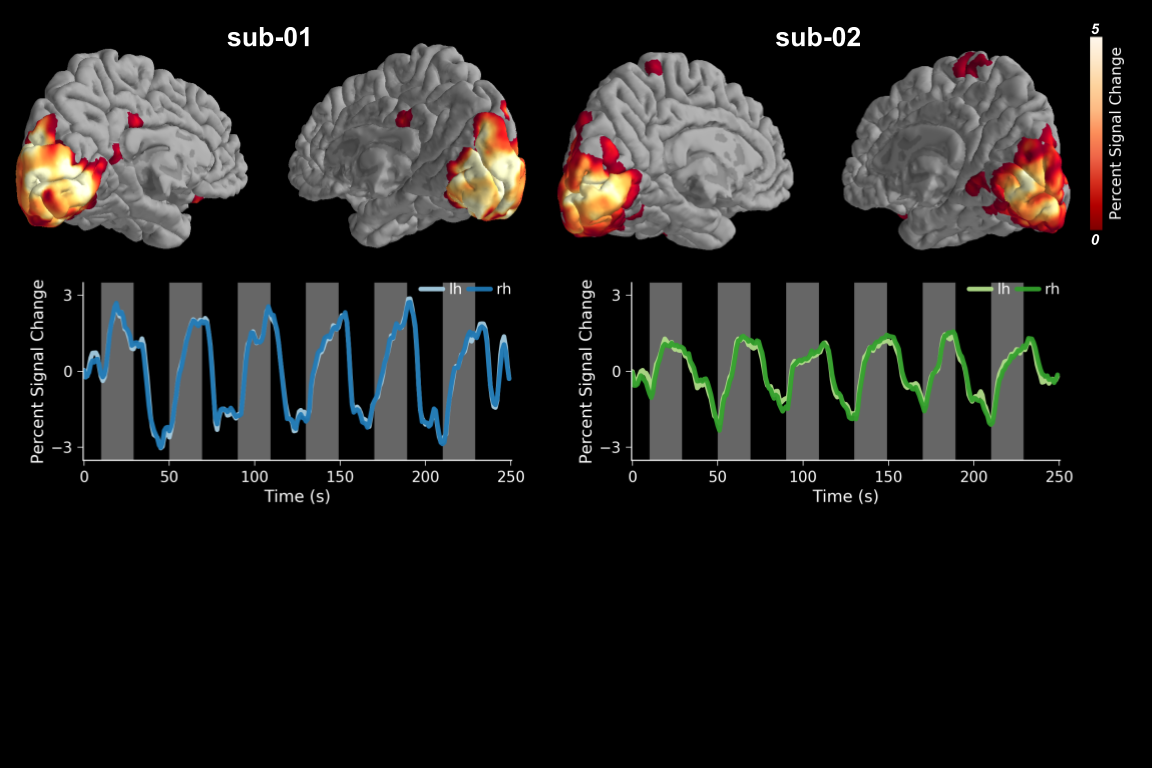
\includegraphics[trim={0 9cm 0 0},clip]{fig1.png}}%
}
\caption{\textbf{BOLD signal in response to visual stimulation}}
\par Top: Percent signal change maps. Thresholded only to significant voxels using permutation testing (5000 iterations) and FWE correction. Bottom: Timecourses for voxels from largest cluster for each participant \& hemisphere.
\end{figure}

Next, the effects of task-correlated respiratory artifact was measured in the presence of a hypercapniac and hypocapniac (breath-holding and hyperventilation, respectively). When the response to visual stimulation was measured without accounting for breath-holding, significant BOLD activation was detected across the cortex (Figure 2a / S1a). Conversely, when the response to visual stimulation was measured without accounting for hyperventilation, significant BOLD deactivation was detected across the cortex (Figure 2b / S1b). These results show a significant reduction in detection power (defined as accuracy in correctly estimating BOLD changes where there is, not not where there isn’t) in the presence of uncontrolled respiratory-artifact. 

\subsection{Task-Correlated Respiratory Artifact}
Averaged whole-brain responses to respiratory events, with their corresponding respiratory recordings, are presented in Figure 3. Consistent with previous reports, the BOLD response to a hypercapniac event (breath-holding) is characterized by an initial reduction in percent signal change followed by robust, prolonged increase peaking between 25s to 30s, and decreasing thereafter. Conversely,  the BOLD response to a hypocapniac event (hyperventilation) is nearly the exact opposite: an initial increase in percent signal change followed by robust, prolonged decrease peaking around 25s and recovering slowly thereafter. 

\begin{figure}
\centerline{%
\resizebox{1.0\textwidth}{!}{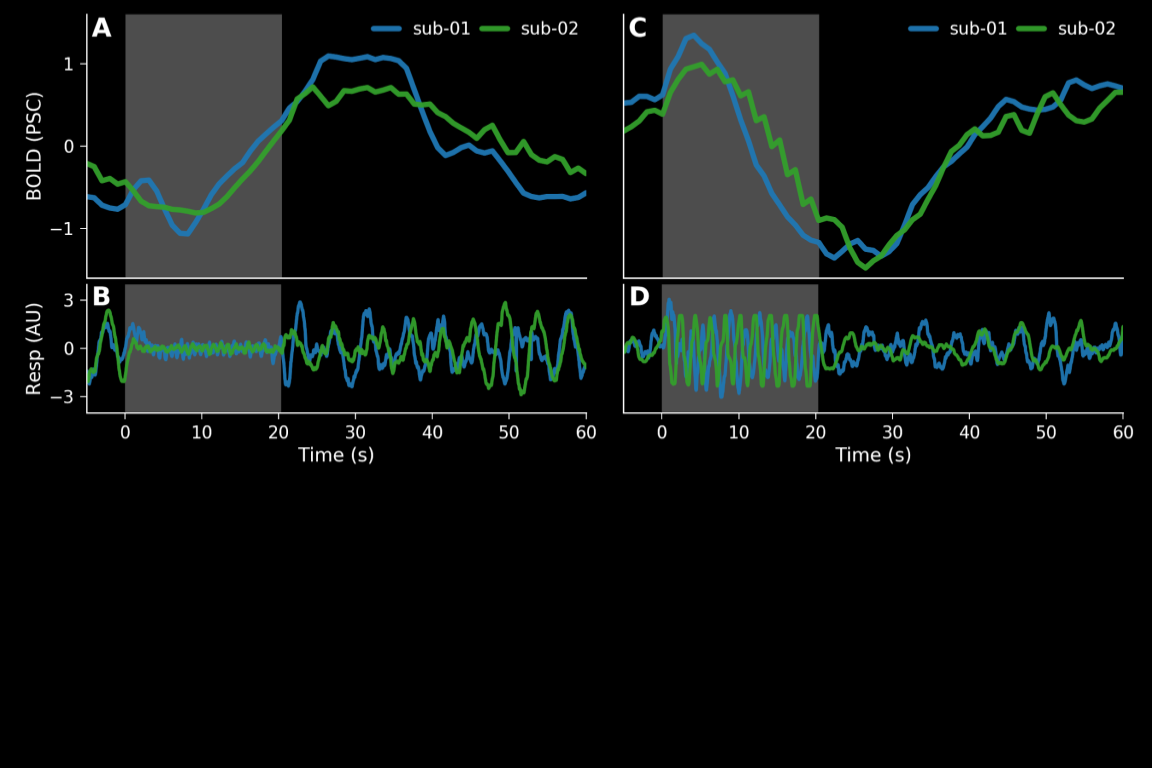
\includegraphics[trim={0 10.2cm 0 0},clip]{fig2.png}}%
}
\caption{\textbf{Respiratory Event Waveform}}

\end{figure}

Next, testing for estimation power. Using the visual cortex maps defined above, we extracted the average percent signal change to visual stimulation in both the breath-holding and hyperventilation conditions. Collapsing across hemispheres, pairwise contrasts were computed to estimate the effects of respiratory events on visual stimulation. Except in one instance, the estimated BOLD response in visual cortex to visual stimulation was significantly reduced in the presence of both types of respiratory events (sub-01 control vs. breath-holding: F = 0.04, p = 0.848; sub-01 control vs. hyperventilation: F = 38.19, p < 0.001; sub-02 control vs. breath-holding: F = 24.45, p < 0.001; sub-02 control vs. hyperventilation: F = 20.94, p < 0.001). 

\begin{figure}
\centerline{%
\resizebox{1.0\textwidth}{!}{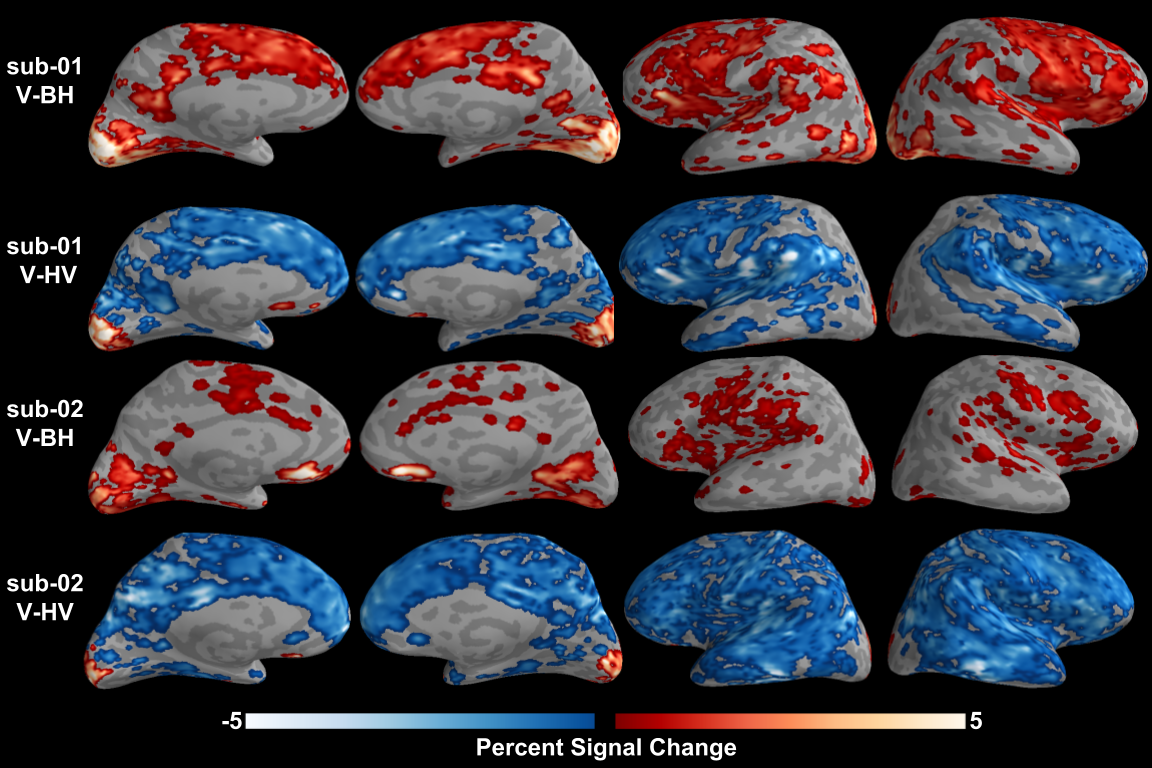
\includegraphics{fig3.png}}%
}
\caption{\textbf{Task-correlated respiratory artifact}}

\end{figure}

NOTE ANATOMICAL VARIABILITY IN BOLD CHANGE

In summary, task-correlated respiratory artifact, when uncontrolled for, can result in substantially reduced detection power (i.e. increase in false positives) and estimation power (i.e. significant reduction of true effects). 

\subsection{Correcting for Task-Correlated Respiration}

\begin{figure}
\centerline{%
\resizebox{1.0\textwidth}{!}{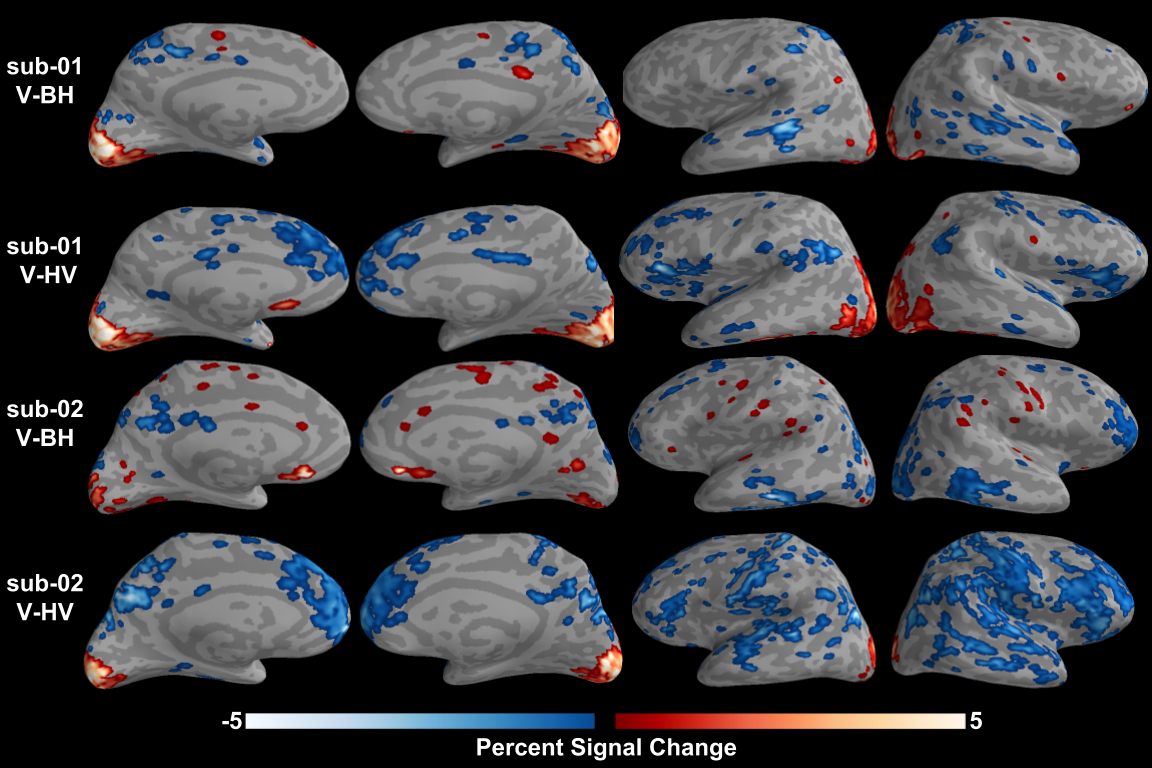
\includegraphics{fig4.png}}%
}
\caption{\textbf{Correcting for artifact with CompCor}}

\end{figure}

\begin{figure}
\centerline{%
\resizebox{1.0\textwidth}{!}{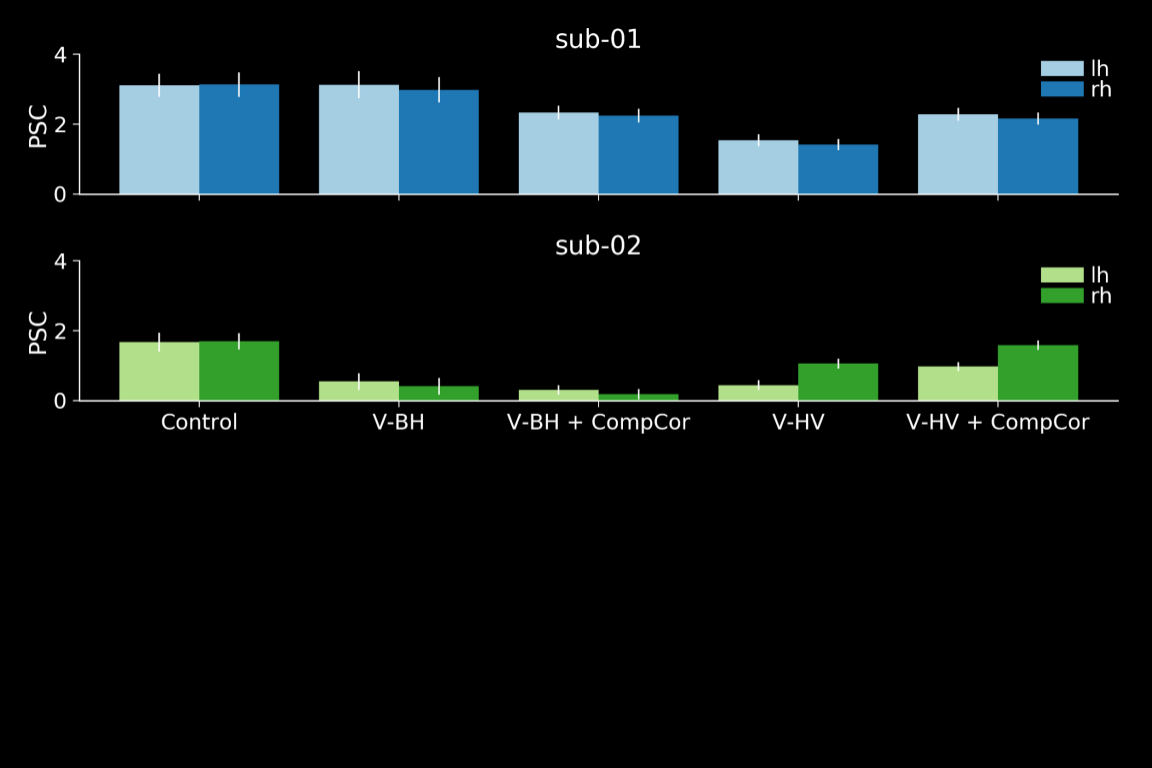
\includegraphics[trim={0 11cm 0 0},clip]{fig5.png}}%
}
\caption{\textbf{Respiratory Event Waveform}}

\end{figure}

\section{Discussion}

\section{Methods}

\subsection{Participants}
All experimental procedures were approved by the NEU502b course instructors. Two participants (both female, age 25) volunteered to participate in this experiment as part of a course on cognitive neuroscience methods. Both participants reported being right-handed and without a current or past diagnosis of a psychiatric or neurological disorder.

\subsection{Task Paradigms}
(Birn et al., 2009; Bright et al., 2009) 

\textbf{Visual Stimulation} The visual localizer task was used to detect BOLD response visual cortex. To evoke a BOLD response, participants viewed a rotating and flashing black-and-white checkerboard stimulus. Each stimulus lasted 20 s followed by 20 s of fixation. The checkerboard stimulus was presented six total times. The run lasted 250 s.

\textbf{Breathhold} The breathholding task was used to measure the physiological BOLD response to a hypercapniac event. Participants were instructed to hold their breath for 20 s, followed by a recovery period of 40 s. Participants completed six total trials of breathholding. The run lasted 370 s.

\textbf{Hyperventilate} The hyperventilation task was used to measure the physiological BOLD response to a hypocapniac event. Participants were coached rapidly inhale then exhale, with each action lasting 2 s. This was followed by a recovery period of 40 s. Participants completed six total trials of hyperventilation. The run lasted 370 s.

\textbf{Visual Breathhold} The visual-breathhold task was designed to measure the effects of a hypercapniac event on BOLD detection in visual cortex. Participants were again instructed to hold their breath for 20 s. After 10 s elapsed, the same checkerboard stimuli as above were presented for 20 s such that breathholding ended 10 s into the presentation of the visual stimulus. Blocks of breathholding and visual stimuli were separated by 30 s of fixation. The run lasted 370 s.

\textbf{Visual Hyperventilate} The visual-hyperventilation task was designed to measure the effects of a hypocapniac event on BOLD detection in visual cortex. Participants were again coached in rapid breathing for 20 s. After 10 s elapsed, the same checkerboard stimuli as above were presented for 20 s such that hyperventilation ended 10 s into the presentation of the visual stimulus. Blocks of hyperventilation and visual stimuli were separated by 30 s of fixation. The run lasted 370 s.

Visual stimuli were programmed in Python and Psychopy(Peirce, 2008) and were presented with a projector. Participants viewed the projection on a screen fixed at the back of the scanner bore, through a mirror fixed in front of the eyes.

\subsection{Data Acquisition}
Briefly, all images were acquired with a 64 channel head coil on a 3T Siemens Prisma. A T1-weighted MPRAGE image was acquired with TR=2530 ms,  TE 3.31 ms, flip angle=7 deg, in-plane FOV=256 x 256 mm, 176 slices, 1.0 mm isotropic voxels. For advanced anatomical registration (see below), a T2-weighted image was acquired TR=3200 ms, TE=428 ms, flip angle=120 deg, in-plane FOV=256 × 256 mm, 72 slices, 1.0 mm isotropic voxels. Whole-brain EPI acquisitions were acquired with TR=1000 ms, TE=30 ms, flip angle=55 deg, in-plane FOV=192 × 192 mm, 56 slices, 3.0 mm isotropic voxels, with a multi-band acceleration factor of 4. One run of each task was acquired with anterior-to-posterior phase encoding. Prior to the collection of the EPI images, a fieldmap was acquired for the purposes of susceptibility distortion correction (see below) with TR=1000 ms, TE=3.47 ms, flip angle=120 deg, in-plane FOV=192 × 192 mm, 56 slices, 3.0 mm isotropic voxels.

To measure cardiac and respiratory signals, a pulse oximeter and respiratory bellows were fitted to participants prior to the scanning. The pulse and respiratory signals were recorded by the scanner host computer at a sampling rate of 200 Hz and 50 Hz, respectively. The recordings were aligned with the onset of the first sync pulse using a custom script. 

\subsection{Data Preprocessing}

Results included in this manuscript come from preprocessing performed using FMRIPREP v1.0.8 (Esteban et al., 2018), a Nipype based tool (Gorgolewski et al., 2011, 2017). Each T1w (T1-weighted) volume was corrected for INU (intensity non-uniformity) using \textit{N4BiasFieldCorrection} v2.1.0  (Tustison et al., 2010) and skull-stripped using \textit{antsBrainExtraction.sh} v2.1.0 (using the OASIS template). Brain surfaces were reconstructed using \textit{recon-all} from FreeSurfer v6.0.0 (Dale et al., 1999), and the brain mask estimated previously was refined with a custom variation of the method to reconcile ANTs-derived and FreeSurfer-derived segmentations of the cortical gray-matter of Mindboggle (Klein et al., 2017). Spatial normalization to the ICBM 152 Nonlinear Asymmetrical template version 2009c (Fonov et al., 2009) was performed through nonlinear registration with the \textit{antsRegistration} tool of ANTs v2.1.0 (Avants et al., 2008), using brain-extracted versions of both T1w volume and template. Brain tissue segmentation of cerebrospinal fluid (CSF), white-matter (WM) and gray-matter (GM) was performed on the brain-extracted T1w using \textit{fast} (FSL v5.0.9) (Zhang et al., 2001).

Functional data was motion corrected using \textit{mcflirt} (FSL v5.0.9; Jenkinson et al., 2002). Slice timing was not performed in light of the task design and short repetition time. Distortion correction was performed using an implementation of the TOPUP technique (Andersson et al., 2003) using \textit{3dQwarp} (AFNI v16.2.07; Cox, 1996). This was followed by co-registration to the corresponding T1w using boundary-based registration (Greve and Fischl, 2009) with 9 degrees of freedom, using \textit{bbregister} (FreeSurfer v6.0.0). Motion correcting transformations, field distortion correcting warp, BOLD-to-T1w transformation and T1w-to-template (MNI) warp were concatenated and applied in a single step using \textit{antsApplyTransforms} (ANTs v2.1.0) using Lanczos interpolation.

Physiological noise regressors were extracted applying CompCor (Behzadi et al., 2007). Principal components were estimated for the two CompCor variants: temporal (tCompCor) and anatomical (aCompCor). A mask to exclude signal with cortical origin was obtained by eroding the brain mask, ensuring it only contained subcortical structures. Six tCompCor components were then calculated including only the top 5\% variable voxels within that subcortical mask. For aCompCor, six components were calculated within the intersection of the subcortical mask and the union of CSF and WM masks calculated in T1w space, after their projection to the native space of each functional run. Framewise displacement (Power et al., 2014) was calculated for each functional run using the implementation of Nipype.

Many internal operations of FMRIPREP use \textit{Nilearn} (Abraham et al., 2014), principally within the BOLD-processing workflow. For more details of the pipeline see \href{https://fmriprep.readthedocs.io/en/latest/workflows.html}{https://fmriprep.readthedocs.io/en/latest/workflows.html}.

Image quality was assessed using MRIQC v0.10.4 (Esteban et al., 2017). Both anatomical and functional scans were visually inspected for artifacts and showed no apparent defects. For completeness, the QC reports, including carpet plots of the raw BOLD signal (Power, 2017), are included for inspection.

\subsection{Data Analysis}
Prior to regression analysis, all functional data were downsampled to the \textit{fsaverage5} template brain (10242 vertices per hemisphere). This 10-fold reduction in mesh vertices is similar to applying spatial smoothing with FWHM of approximately 6 mm\textsuperscript{2}. To remove  low frequency drift terms, functional data were also high-passed filtered at 100s using Nilearn.

Functional activation maps in response to the visual checkerboard stimulus were obtained by regressing each voxel time series against a boxcar function corresponding to the onset/offset times of the stimulus convolved with the canonical hemodynamic response function. In the first analysis (localizer), the ideal task response was modeled in the uncorrupted runs (run 1). In the second analysis, the ideal task response was modeled in the presence of task-correlated respiratory artifact (breath-holding and hyperventilation). In the third analysis,  the ideal task response in the presence of task-correlated respiratory artifact and artifact regressors. In the fourth and final analysis, the ideal task response in the presence of task-correlated respiratory artifact and CompCor regressors.

For all analyses, additional nuisance regressors were included. These included the timeseries of motion, which were demeaned, linearly detrended, and orthogonalized prior to regression. We also include “motion scrubbers”, which remove volumes with high motion artifact (FD > 0.5) as previously recommended (Power et al., 2014; Siegel et al., 2014). To correct for temporal autocorrelation, the data and design matrices were prewhitened using a Tukey taper approach (Woolrich et al., 2001). Multiple comparisons corrections were implemented through permutation testing with 5000 null iterations and family-wise error correction at alpha = 0.05 (Winkler et al., 2014). Final results projected back onto native freesurfer brains for visualization. 

\nocite{*} % This command displays all refs in the bib file. PLEASE DELETE IT BEFORE YOU SUBMIT YOUR MANUSCRIPT!
\bibliography{NEU502b-fmri}

\end{document}